%
\documentclass[12pt]{article}

% usual packages
\usepackage{fullpage}
\usepackage{setspace}
\usepackage{graphicx}
\usepackage{float}
\usepackage{amsmath}
\usepackage{amsfonts}
\usepackage{amssymb}

% bibliography and references
\usepackage{natbib}
\bibpunct{(}{)}{;}{a}{}{,}

% set paragraph spacing the way I like
\parskip=0pt
\parindent=20pt

% remove indent from footnotes
%\usepackage[hang,flushmargin]{footmisc}

% style font beneath figures
\usepackage[labelfont={bf}, margin=0cm, font=small, skip=0pt]{caption}

% create footnote command so that my name
% has an asterisk rather than a one.
\long\def\symbolfootnote[#1]#2{\begingroup%
\def\thefootnote{\fnsymbol{footnote}}\footnote[#1]{#2}\endgroup}

% body font
\usepackage[T1]{fontenc}
\usepackage{newtxtext,newtxmath}


% pdf meta data and link styling
\usepackage{hyperref}
\hypersetup{
 pdftitle={Estimating Logit Models with Small Samples}, % title
 pdfauthor={Kelly McCaskey and Carlisle Rainey}, % author
 pdfkeywords={logit}{probit}{logistic regression} {small sample} {bias},
 pdfnewwindow=true, % links in new window
 colorlinks=true, % false: boxed links; true: colored links
 linkcolor=black, % color of internal links
 citecolor=black, % color of links to bibliography
 filecolor=black, % color of file links
 urlcolor=blue % color of external links
}

%% enable comments in pdf
%\newcommand{\kelly}[1]{\textcolor{blue}{#1}}
%\newcommand{\carlisle}[1]{\textcolor{magenta}{#1}}


\begin{document}

\begin{center}
{\LARGE{\textbf{Estimating Logit Models with Small Samples}}\symbolfootnote[1]{We thank Tracy George, Lee Epstein, and Alex Weisiger for making their data available.
%We thank Scott Cook, Paul Kellstedt, Dan Wood, Chris Zorn, and participants at the 2015 Annual Meeting of the Society for Political Methodology and a seminar at Texas A&M University for helpful comments.
We conducted these analyses analyses with \texttt{R} 3.2.2.
All data and computer code necessary for replication are available at \href{https://www.github.com/kellymccaskey/small}{github.com/kellymccaskey/small}.}}\\\vspace{2mm}

\vspace{10mm}

Kelly McCaskey\symbolfootnote[2]{Kelly McCaskey is a Ph.D. student in the Department of Political Science, Texas A\&M University, 2010 Allen Building, College Station, TX, 77843 (\href{mailto:kellymccaskey@tamu.edu}{kellymccaskey@tamu.edu}).}

\vspace{3mm}

Carlisle Rainey\symbolfootnote[3]{Carlisle Rainey is Assistant Professor of Political Science, Texas A\&M University, 2010 Allen Building, College Station, TX, 77843 (\href{mailto:crainey@tamu.edu}{crainey@tamu.edu}).}
\end{center}

\vspace{10mm}

% Abstract
{\centerline{\textbf{Abstract}}}
\begin{quote}\noindent
In small samples, maximum likelihood (ML) estimates of logit model coefficients have substantial bias away from zero.
As a solution, we introduce political scientists to the penalized maximum likelihood (PML) estimator \citep{Firth1993}.
The PML estimator eliminates most of the bias and, perhaps more importantly, greatly reduces the variance of the usual ML estimator.
Thus, researchers do not face a bias-variance tradeoff when choosing between the ML and PML estimators--the PML estimator has a smaller bias \textit{and} a smaller variance and the reductions are substantial in small samples.
Monte Carlo simulations and a re-analysis of \cite{GeorgeEpstein1992} show that PML estimates significantly improve upon ML estimates.
 \end{quote}

 \vspace{5mm}
 \begin{center}
 Word Count: 8,011
 \end{center}

% Remove page number from first page
\thispagestyle{empty}

% Start main text
\newpage
\doublespace

% set the context
Logit and probit models have become a staple in quantitative political and social science--nearly as common as linear regression \citep{KruegerLewisBeck2008}. 
Political scientists typically rely on maximum likelihood (ML) to estimate these models.
While ML estimates have excellent large-sample properties, the ML estimates of logit and probit model coefficients behave quite poorly in small samples.

\section*{The Big Problem with Small Samples}

When working with a binary outcome $y_i$, the researcher typically models probability of an event, so that
\begin{equation}\label{eqn:pry}
\text{Pr}(y_i) = \text{Pr}(y_i = 1~|~ X_i) =  g^{-1}(X_i\beta)\text{ ,}
\end{equation}
where $y$ represents a vector of binary outcomes, $X$ represents a matrix of explanatory variables and a constant, $\beta$ represents a vector of model coefficients, and $g^{-1}$ represents some inverse-link function that maps $\mathbb{R}$ into $[0, 1]$. 
When $g^{-1}$ represents the inverse-logit function $\text{logit}^{-1}(\alpha) = \dfrac{1}{1 + e^{-\alpha}}$ or the cumulative normal distribution function $\Phi(\alpha) = \int_{-\infty}^\alpha \frac{1}{\sqrt{2\pi}}e^{-\frac{x^2}{2}}dx$, then we refer to Equation \ref{eqn:pry} as a logit or probit model, respectively.
To simplify the exposition, we focus on logit models, because the canonical logit link function induces nicer theoretical properties \citep[pp. 31-32]{McCullaghNelder1989}. 
In practice, though, \cite{KosmidisFirth2009} shows that the ideas we discuss applies equally well to probit models.

To develop the ML estimator of the logit model, we can derive the likelihood function
\begin{equation}\nonumber
\text{Pr}(y | \beta) = L(\beta | y) = \displaystyle \prod_{i = 1}^n \left[\left( \dfrac{1}{1 + e^{-X_i\beta}}\right)^{y_i}\left(1- \dfrac{1}{1 + e^{-X_i\beta}}\right)^{1 - y_i}\right]\text{.}
\end{equation}
\noindent As usual, we take the natural logarithm of both sides to obtain the log-likelihood function
\begin{equation}\nonumber
\log L(\beta | y) = \displaystyle \sum_{i = 1}^n \left[y_i \log \left( \dfrac{1}{1 + e^{-X_i\beta}}\right) + (1 - y_i) \log \left(1- \dfrac{1}{1 + e^{-X_i\beta}}\right)\right].
\end{equation}
\noindent The researcher can find the ML estimate $\hat{\beta}^{mle}$ by finding the vector $\beta$ that maximizes $\log L$ \citep{King1989}.

The ML estimate of the logit model coefficient vector $\hat{\beta}^{mle}$ is asymptotically unbiased, so that $E(\hat{\beta}^{mle}) \approx \beta^{true}$ when the sample is large (\citealt{Wooldridge2002}, pp. 391-395, and \citealt{CasellaBerger2002}, p. 470), and asymptotically efficient, so that the asymptotic variance of the ML estimate equals the Cramer-Rao lower bound (\citealt{Greene2012}, pp. 513-523, and \citealt{CasellaBerger2002}, pp. 472, 516). 
For small samples, though, the ML estimator of logit model coefficients does not work well--the ML estimates have substantial bias away from zero \citep[pp. 53-54]{Long1997}.

\citet[p. 54]{Long1997} offers a rough heuristic about appropriate sample sizes: ``It is risky to use ML with samples smaller than 100, while samples larger than 500 seem adequate.''\footnote{Making the problem worse, \cite{KingZeng2001} point out that ML estimates have substantial bias for much larger sample sizes if the event of interest occurs only rarely.}
This presents the researcher with a problem: When dealing with small samples, how can she obtain reasonable estimates of logit model coefficients?

\section*{An Easy Solution for the Big Problem}

The statistics literature offers a simple solution to the problem of bias.
\cite{Firth1993} suggests penalizing the usual likelihood function $L(\beta | y)$ by a factor equal to the square root of the determinant of the information matrix $|I(\beta)|^\frac{1}{2}$, which produces a ``penalized'' likelihood function $L^*(\beta | y) = L(\beta | y)|I(\beta)|^\frac{1}{2}$ (see also \citealt{KosmidisFirth2009} and \citealt{Kosmidis2014}).
It turns out that this penalty is equivalent to Jeffreys' (\citeyear{Jeffreys1946}) prior for the logit model (\citealt{Firth1993} and \citealt{Poirier1994}).
We take the natural logarithm of both sides to obtain the \textit{penalized} log-likelihood function.
\begin{equation}\nonumber
\log L^*(\beta | y) = \displaystyle \sum_{i = 1}^n \left[y_i \log \left( \dfrac{1}{1 + e^{-X_i\beta}}\right) + (1 - y_i) \log \left(1 - \dfrac{1}{1 + e^{-X_i\beta}}\right)\right] + \dfrac{1}{2} \log |I(\beta)|.
\end{equation}
Then the researcher can find the penalized maximum likelihood (PML) estimate $\hat{\beta}^{pmle}$ by finding the vector $\beta$ that maximizes $\log L^*$.
\cite{Zorn2005} suggested PML for solving the problem of separation,
% (see also \citealt{Rainey-separation})
but the broader and perhaps more important application to small sample problems seems to remain unnoticed in political science.

A researcher can implement PML as easily as ML, but PML estimates of logit model coefficients have a smaller bias \citep{Firth1993} and a smaller variance (\citealt[p. 49]{Kosmidis2007}, and \citealt{Copas1988}).\footnote{The penalized maximum likelihood estimates are easy to calculate in R using the \texttt{logistf} or \texttt{brglm} packages and in Stata with the \texttt{firthlogit} module. 
See the Section \ref{sec:pmle-in-R} and Section \ref{sec:pmle-in-stata} of the Appendix, respectively, for examples.}
This is important.
When choosing among estimators, researchers often face a tradeoff between bias and variance \citep[pp. 37-38]{HastieTibshiraniFriedman2013}, but \textit{there is no bias-variance tradeoff between ML and PML estimators}.
The PML estimator exhibits both lower bias \textit{and} lower variance.

Two concepts from statistical theory illuminate the relationship between the ML and PML estimators. 
Suppose two estimators $A$ and $B$, with a quadratic loss function so that the risk functions $R^A$ and $R^B$ (i.e., the expected loss) corresponds to the mean-squared error (MSE). 
If $R^A \leq R^B$ for all parameter values and the inequality holds strictly for at least some parameter values, then we can refer to estimator $B$ as \textit{inadmissible} and say that estimator $A$ \textit{dominates} estimator $B$ (\citealt{DeGrootSchervish2012}, p. 458, and \citealt{LeonardHsu1999}, pp. 143-146). 
Now suppose a quadratic loss function for the logit model coefficients, such that $R^{mle} = E[(\hat{\beta}^{mle} - \beta^{true})^2]$ and $R^{pmle} = E[(\hat{\beta}^{pmle} - \beta^{true})^2]$. 
In this case, the inequality holds strictly for all $\beta^{true}$ so that $R^{pmle} < R^{mle}$. Thus, we can describe the ML estimator as \textit{inadmissible} and say that the PML estimator \textit{dominates} the ML estimator.

The intuition of the bias reduction is subtle. 
First, consider the source of the bias.
Calculate the score function $s$ as the gradient (or first-derivative) of the log-likelihood with respect to $\beta$ so that $s(y, \beta) = \nabla \log L(\beta | y)$. 
(Note that solving $s(y, \hat{\beta}^{mle}) = 0$ is equivalent to finding $\hat{\beta}^{mle}$ that maximizes $\log L(\beta | y)$.) 
Now recall that at the true parameter vector $\beta^{true}$, the expected value of the score function is zero so that $E\left[ s(y, \beta^{true})\right] = 0$ \citep[p. 517]{Greene2012}.
This implies that $E\left[ s(y, \beta^{true}) | s(y, \beta^{true}) > 0 \right] =  E\left[ s(y, \beta^{true}) | s(y, \beta^{true}) < 0 \right]$--that high and low misses cancel exactly.
However, if the score function $s$ is curved in the area around $\beta^{true}_j$ so that $s''_j = \frac{\partial^2 s(y, \beta)}{\partial^2 \beta_j} > 0$, then $s(y, \beta^{true}) > 0$ generates large misses to the right of $\beta^{true}_j$ and $s(y, \beta^{true}) < 0$ generates small misses to the left of $\beta^{true}_j$. 
Similarly, if $s''_j < 0$, then $s(y, \beta^{true}) > 0$ generates small misses to the right of $\beta^{true}_j$ and $s(y, \beta^{true}) < 0$ generates large misses to the left of $\beta^{true}_j$. 
The large and small misses do not cancel out, so that $E(\hat{\beta}^{mle}_j) > \beta^{true}_j$ when $s''_j > 0$ and $E(\hat{\beta}^{mle}) < \beta^{true}_j$ when $s''_j < 0$.
\citet[pp. 251-252]{CoxSnell1968} derive a formal statement of this bias of order $n^{-1}$, which we denote as $\text{bias}_{n^{-1}}(\beta^{true})$. 

Now consider the bias reduction strategy. 
At first glance, one may simply decide to subtract the bias $\text{bias}_{n^{-1}}(\beta^{true})$ from the estimate $\hat{\beta}^{mle}$. 
However, note that the bias depends on the true parameter. 
Because researchers do not know the true parameter, this is not a viable strategy, though \cite{AndersonRichardson1979} explore the option of correcting the bias by using  $\hat{\beta}^{mle} - \text{bias}_{n^{-1}}(\hat{\beta}^{mle})$.
However, \cite{Firth1993} suggests modifying the score function, so that $s^*(y, \beta) = s(y, \beta) - \gamma(\beta)$, where $\gamma$ shifts the score function upward or downward.
\cite{Firth1993} shows that one good choice $\gamma$ takes $\gamma_j = \frac{1}{2} \text{trace} \left[ I^{-1} \left( \frac{\partial I}{\partial \beta_j}\right)\right] = \frac{\partial}{\partial \beta_j} \left( \log | I(\beta) | \right)$.
Integrating, we can see that solving $s^*(y, \hat{\beta}^{pmle}) = 0$ is equivalent to finding $\hat{\beta}^{pmle}$ that maximizes $\log L^*(\beta | y)$ with respect to $\beta$.

We can say that the PML estimator dominates the ML estimator because the PML estimator has lower bias and variance \textit{regardless of the sample size}--the PML estimator always outperforms the ML estimator, and least in terms of the bias, variance, and MSE.
However, both estimators are asymptotically unbiased and efficient, so the difference between the two estimators becomes negligible as the sample size grows large.
In small samples, though, Monte Carlo simulations show substantial improvements that should grab the attention of substantive researchers.

\section*{The Big Improvements from an Easy Solution}

To show that the size of reductions in bias, variance, and MSE should draw the attention of substantive researchers, we conduct a Monte Carlo simulation comparing the sampling distributions of the ML and PML estimates.
These simulations demonstrate two features of the ML and PML estimators:
\begin{enumerate}
\item In small samples, the ML estimator exhibits a large bias. The PML estimator is nearly unbiased, regardless of sample size.
\item In small samples, the variance of the ML estimator is much larger than the variance of the PML estimator.
\item The increased bias and variance of the ML estimator implies that the PML estimator will also have a smaller MSE, but importantly, the variance make a much greater contribution to the MSE than the bias.
\end{enumerate}

In our simulation, the true data generating process corresponds to $\Pr(y_i = 1) = \frac{1}{1 + e^{-X_i \beta}}$, where $i \in 1, 2,..., n$ and $X \beta = \beta_{cons} + 0.5 x_1 + \sum_{j = 2}^k 0.2 x_j$, and we focus on the coefficient for $x_1$ as the coefficient of interest.
We draw each fixed $x_j$ from a normal distribution with mean of zero and standard deviation of one and vary the sample size $N$ from 30 to 210, the number of explanatory variables $k$ from 3 to 6 to 9, and the the intercept $\beta_{cons}$ from -1 to -0.5 to 0 (which, in turn, varies the proportion of events $P_{cons}$ from about 0.28 to 0.38 to 0.50).
The biostatistics literature uses the number of events per explanatory variable $\frac{1}{k}\sum y_i$ as a measure of the information in the data set (e.g., \citealt{Peduzzietal1996} and \citealt{VittinghoffMcCulloch2007}), and each parameter of our simulation varies this information, where $ \frac{N \times P_{cons}}{k} \approx \frac{1}{k}\sum y_i$.
For each combination of the simulation parameters, we draw 10,000 data sets and use each data set to estimate the logit model coefficients using ML and PML. 
From these estimates, we compute the percent bias and variance of the ML and PML estimators, as well as the MSE inflation of the ML estimator compared to the PML estimator.

\subsection*{Bias}

We calculate the percent bias $= 100 \times \left(\frac{E(\hat{\beta})}{\beta^{true}} - 1 \right)$ as the intercept $\beta_{cons}$, the number of explanatory variables $k$, and the sample size $N$ vary.
Figure \ref{fig:sims-coef-perc-bias} shows the results.
The sample size varies across the horizontal-axis of each plot and each panel shows a distinct combination of intercept and number of variables in the model.
Across the range of the parameters of our sample, the bias of the MLE varies from about 120\% ($\beta_{cons} = -1$, $k = 9$, and $N = 30$) to around 2\% ($\beta_{cons} = 0$, $k = 3$, and $N = 210$).
The bias in the PMLE, on the other hand, is much smaller.
For the worst-case scenario ($\beta_{cons} = -1$, $k = 9$, and $N = 30$), the ML estimate has an upward bias of about 120\%, while the PML estimate has an upward bias of only about 7\%.\footnote{Figures \ref{fig:ev} and \ref{fig:bias} in Section \ref{sec:app-sims} of the Appendix show the expected value and (absolute) bias of these estimates.}

\begin{figure}[h]
\begin{center}
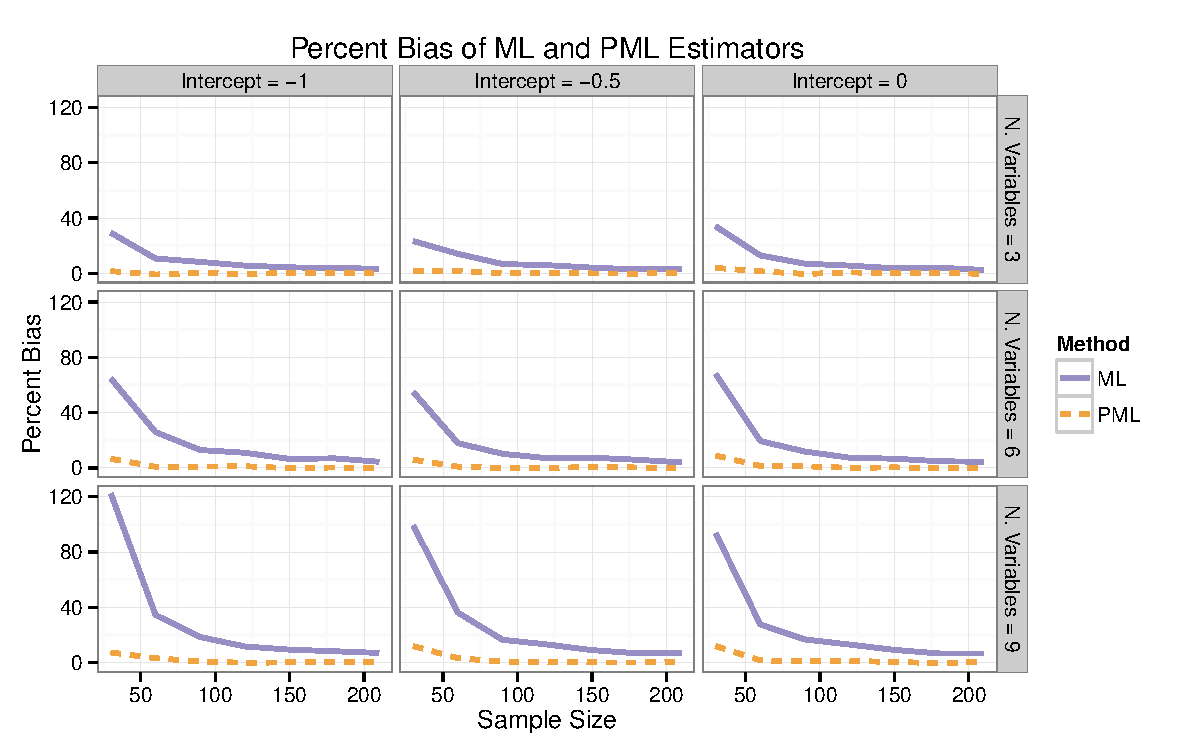
\includegraphics[width = \textwidth]{figs/sims-percent-bias.pdf}
\caption{This figure illustrates the substantial bias of $\hat{\beta}^{mle}$ and the near unbiasedness of $\hat{\beta}^{pmle}$.}\label{fig:sims-coef-perc-bias}
\end{center}
\end{figure}

\subsection*{Variance}

In many cases, estimators trade off bias and variance, but the PML estimator reduces both.
In addition to nearly eliminating the bias, Figure \ref{fig:sims-var} shows that the PML estimator also substantially reduces the variance, especially for the smaller sample sizes.
For $\beta_{cons} = -1$ and $N = 30$, the variance of the ML estimator is about 95\%, 243\%, and 610\% larger than the PML estimator for 3, 6, and 9 variables, respectively.
Doubling the sample size to $N = 60$, the variance remains about 30\%, 58\% and 91\% larger, respectively. 
Even for a larger sample of $N = 210$, the variance of the ML estimator is about 7\%, 10\%, and 14\% larger than the PML estimator.\footnote{Figure \ref{fig:var-infl} in the Appendix shows the variance inflation $= 100 \times \left(\frac{Var(\hat{\beta} ^{mle})}{Var(\hat{\beta}^{pmle})} - 1\right)$.}

\begin{figure}[h]
\begin{center}
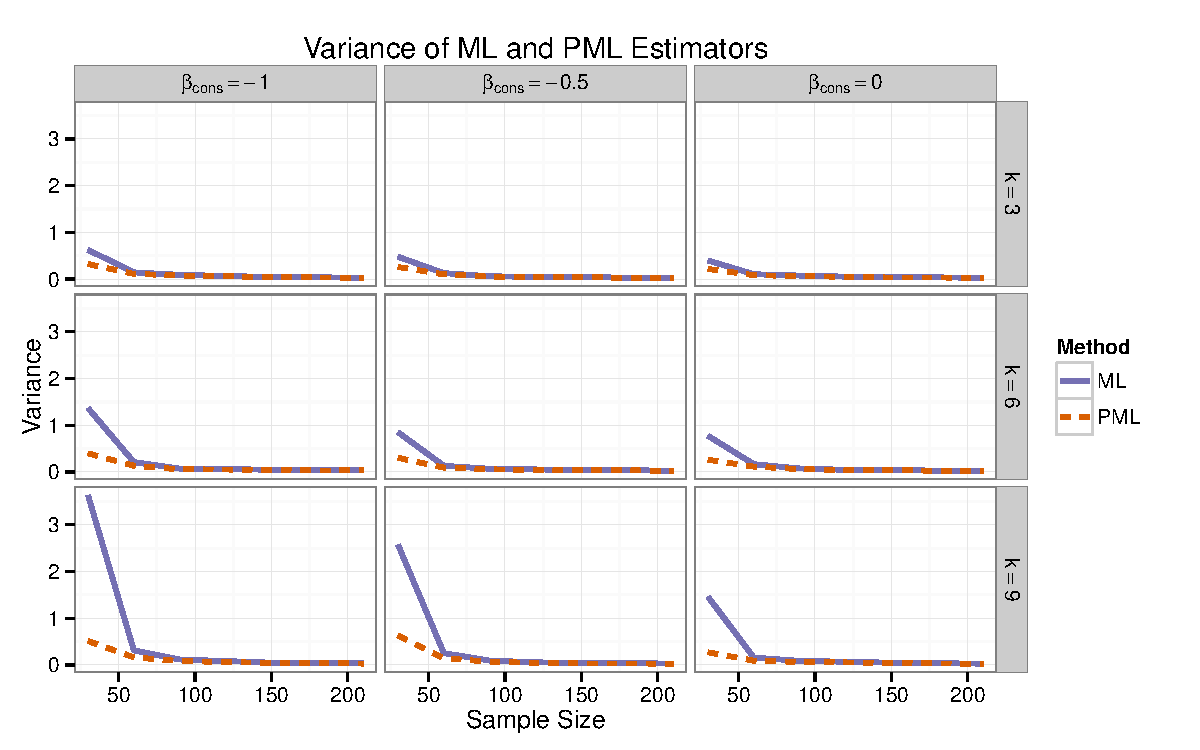
\includegraphics[width = \textwidth]{figs/sims-var.pdf}
\caption{This figure illustrates the smaller variance of $\hat{\beta}^{pmle}$ compared to $\hat{\beta}^{mle}$.}\label{fig:sims-var}
\end{center}
\end{figure}

\subsection*{Mean-Squared Error}

However, neither the bias nor the variance serves as a complete summary of the performance of an estimator.
The MSE, though, combines the bias and variance into an overall measure of the accuracy, where
\begin{align}\label{eqn:mse}
MSE(\hat{\beta}) &= E[(\hat{\beta} - \beta^{true})^2] \nonumber\\
                            &= Var(\hat{\beta}) + [E(\hat{\beta})]^2 \text{.}
\end{align}
Since the bias and the variance of ML estimators exceed the bias and variance the PML estimator, the ML estimator must have a larger MSE, so that $MSE(\hat{\beta}^{mle}) - MSE(\hat{\beta}^{pmle}) > 0$.

We care about the magnitude of this difference, though, not the sign.
To summarize the magnitude of the difference, we compute the percent increase in the MSE for the ML estimator compared to the PML estimator. 
We refer to this quantity as the ``MSE inflation,'' where
\begin{equation}\label{eqn:mse-infl}
\text{MSE inflation} = 100 \times \dfrac{MSE(\hat{\beta}^{mle}) - MSE(\hat{\beta}^{pmle})}{MSE(\hat{\beta}^{pmle})}  \text{ .}
\end{equation}
An MSE inflation of zero indicates that the ML and PML estimators perform equally well, but because the PML estimator dominates the ML estimator, the MSE inflation is strictly greater than zero.
Figure \ref{fig:mse-infl} shows the MSE inflation for each combination of the parameter simulations on the log$_{10}$ scale.
Notice that for the worst-case scenario ($\beta_{cons} = -1$, $k = 9$, and $N = 30$), the MSE of the ML estimates is about 681\% larger than the MSE of the PML estimates.
The MSE inflation only barely drops below 10\% for the most information-rich parameter combinations (e.g., $\beta_{cons} = 0$, $k = 3$, and $N = 210$).
The MSE inflation exceeds 100\% for about 13\% of the simulation parameter combinations, 50\% for about 24\% of the combinations, and 25\% for about 49\% of the combinations.
These large sacrifices in MSE should command the attention of researchers working with binary outcomes and small data sets.

\begin{figure}[h]
\begin{center}
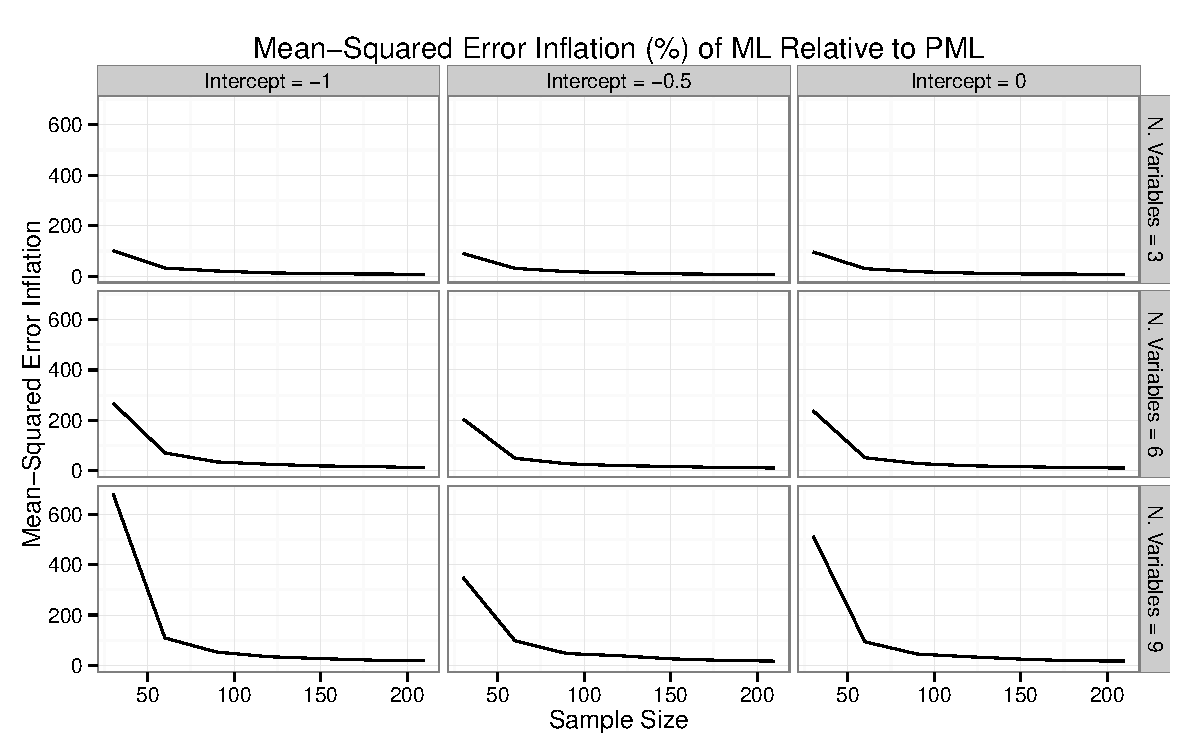
\includegraphics[width = \textwidth]{figs/sims-mse-infl.pdf}
\caption{This figure shows the percent increase in the mean-squared error of $\hat{\beta}^{mle}$ compared to $\hat{\beta}^{pmle}$.}\label{fig:mse-infl}
\end{center}
\end{figure}

However, the larger bias and variance of the ML estimator do not contribute equally to the MSE inflation.
Substituting Equation \ref{eqn:mse} into Equation \ref{eqn:mse-infl} for $MSE(\hat{\beta}^{mle})$ and $MSE(\hat{\beta}^{pmle})$ and rearranging, we obtain
\begin{equation}
\text{MSE inflation} = \overbrace{100 \times \dfrac{Var(\hat{\beta})}{Var(\hat{\beta}^{pmle}) + [E(\hat{\beta}^{pmle})]^2}}^{\text{contribution of variance}} + \overbrace{100 \times \dfrac{[E(\hat{\beta})]^2}{Var(\hat{\beta}^{pmle}) + [E(\hat{\beta}^{pmle})]^2}}^{\text{contribution of bias}}  + 100 \text{ ,} \nonumber
\end{equation}
\noindent which additively separates the contribution of the bias and variance to the MSE inflation.
If we wanted, we could simply plug in the simulation estimates of the bias and variance of each estimator to obtain the contribution of each.
But notice that we can easily compare the \textit{relative} contributions of the bias and variance using the ratio
\begin{equation}\label{eqn:rel-contrib}
\text{relative contribution of variance} = \dfrac{\text{contribution of variance}}{\text{contribution of bias}} \text{ .}
\end{equation}
\noindent Figure \ref{fig:relcontrib-n-scatter} shows the relative contribution of the variance.
Values less than one indicate that the bias makes a greater contribution and values greater than one indicate that the variance makes a greater contribution.
In each case, the relative contribution of the variance is much larger than one.
For $N = 30$, the contribution of the variance is between 7 and 36 times larger than the contribution of the bias.
For $N = 210$, the contribution of the variance is between 25 and 180 times larger than the contribution of the bias.
In spite of the attention paid to the small sample \textit{bias} in ML estimates of logit model coefficients, the small sample \textit{variance} is a more important problem to address, at least in terms of the accuracy of the estimator.
Fortunately, the PML estimator greatly reduces the bias \textit{and} variance, resulting in a much smaller MSE, especially for small samples.

\begin{figure}[h]
\begin{center}
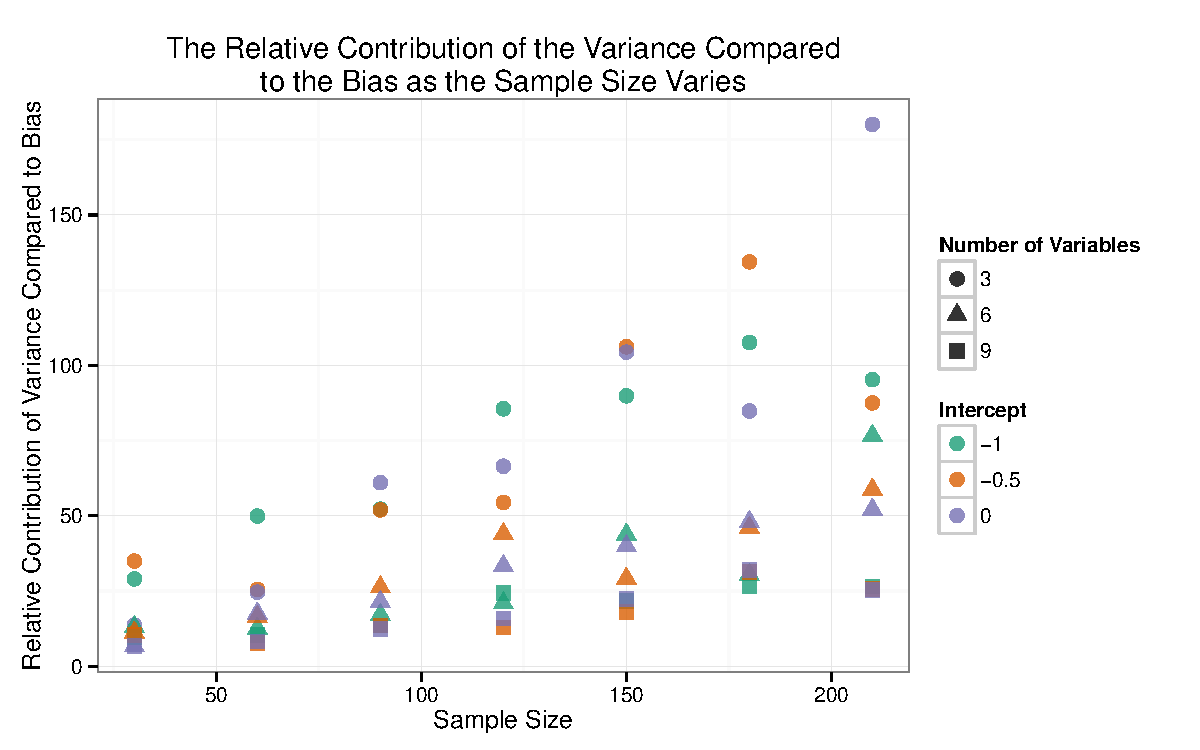
\includegraphics[scale = 0.7]{figs/relcontrib-n-scatter.pdf}
\caption{This figure shows the relative contribution of the variance and bias to the MSE inflation. The relative contribution is defined in Equation \ref{eqn:rel-contrib}.}\label{fig:relcontrib-n-scatter}
\end{center}
\end{figure}

These simulation results show that the bias, variance, and MSE of the ML estimates of logit model coefficients are not trivial in small samples.
Researchers cannot safely ignore these problems.
Fortunately, researchers can implement the PML estimator with little to no added effort and obtain substantial improvements over the usual ML estimator. 
And these improvements are not limited to Monte Carlo studies. 
In the two example application that followa, we show that the PML estimator leads to substantial reductions in the magnitude of the coefficient estimates and in the width of the confidence intervals.

\section*{The Substantive Importance of the Big Improvements}

To illustrate the substantive importance of using the PML estimator, we reanalyze a portion of the statistical analysis in \cite{GeorgeEpstein1992}.\footnote{In Section \ref{app:weisiger} of the Appendix, we include a second re-analysis with similar results.}
We re-estimate the integrated model of U.S. Supreme Court decisions developed by \cite{GeorgeEpstein1992} and find substantial differences in the ML and PML coefficient estimates and the confidence intervals.

\cite{GeorgeEpstein1992} combine the legal and extralegal models of Court decision-making in order to overcome the complementary idiosyncratic shortcomings of each.
The legal model posits \emph{stare decisis}, or the rule of law, as the key determinant of future decisions, while the extralegal model takes a behavioralist approach containing an array of sociological, psychological, and political factors.

The authors model the probability of a conservative decision in favor of the death penalty as a function of a variety of legal and extralegal factors. 
George and Epstein use a small sample of 64 Court decisions involving capital punishment from 1971 to 1988. 
The data set has only with 29 events (i.e., conservative decisions).
They originally use ML to estimate their model and we reproduce their ML estimates exactly.
For comparison, we also estimate the model with the PML estimator that we recommend.
Figure \ref{fig:ge-coefs} shows the coefficient estimates for each method.
In all cases, the PML estimate is smaller than the ML estimate.
Each coefficient decreases by at least 25\% with three decreasing by more than 40\%: court change, the largest, at 49\%, solicitor general at 48\%, and political environment at 41\%.
Additionally, the PML estimator substantially reduces the width of all the confidence intervals.
Three of the 11 coefficients lose statistical significance.

\begin{figure}[h]
\begin{center}
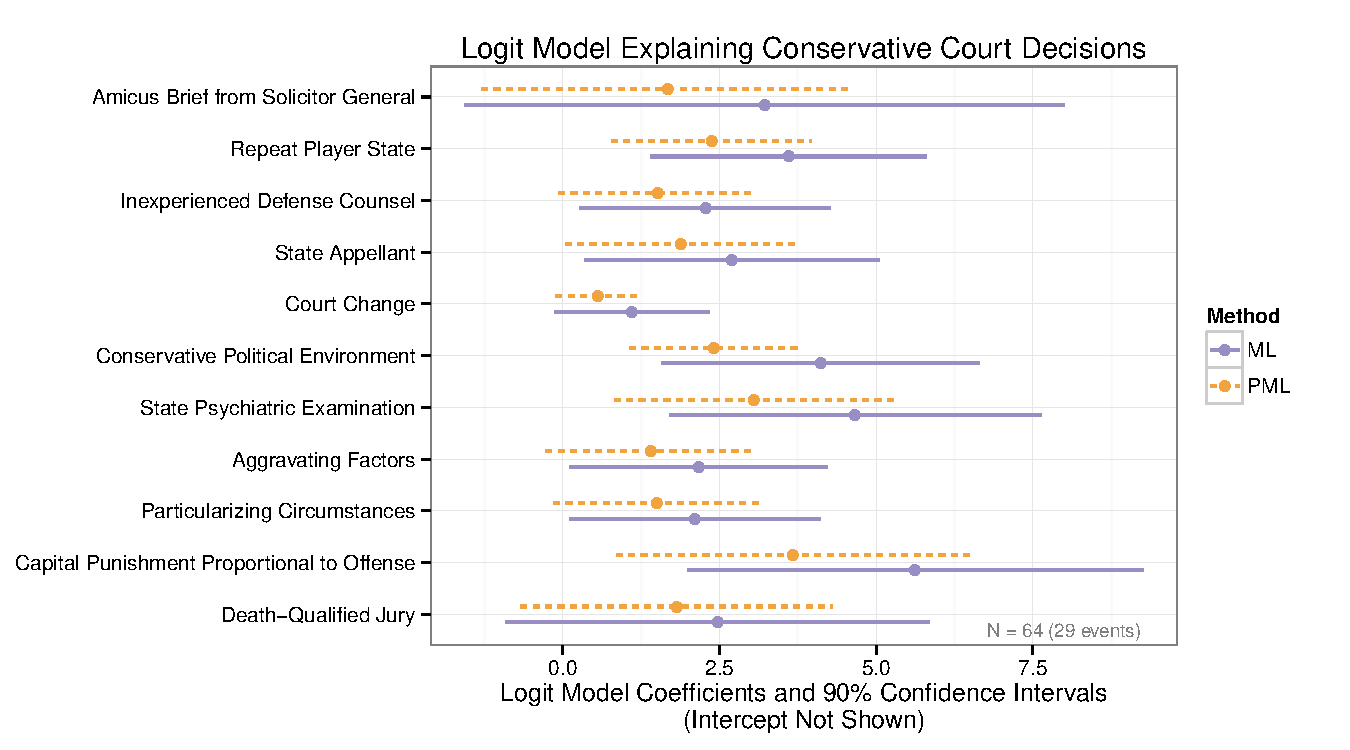
\includegraphics[width = \textwidth]{figs/ge-coefs.pdf}
\caption{This figure shows the coefficients for a logit model model estimating U.S. Supreme Court Decisions by both ML and PML.}\label{fig:ge-coefs}
\end{center}
\end{figure}

Because we do not know the true model, we cannot know which of these sets of coefficients is better.
However, we can use out-of-sample prediction to help adjudicate between these two methods.
We use leave-one-out cross-validation and summarize the prediction errors using Brier and log scores, for which smaller values indicate better predictive ability.\footnote{The Brier score is calculated as $\sum_{i = 1}^n (y_i - p_i)^2$, where $i$ indexes the observations, $y_i \in \{0, 1\}$ represents the actual outcome, and $p_i \in (0, 1)$ represents the estimated probability that $y_i = 1$.
The log score as $-\sum_{i = 1}^n log(r_i)$, where $r_i = y_i p_i + (1 - y_i)(1 - p_i)$.
Notice that because we are logging $r_i \in [0, 1]$, $\sum_{i = 1}^n log(r_i)$ is always negative and smaller (i.e., more negative) values indicate worse fit.
We choose to take the negative of $\sum_{i = 1}^n log(r_i)$, so that, like the Brier score, larger values indicate a worse fit.}
The ML estimates produce a Brier score of 0.17, and the PML estimates lower the Brier score by 8\% to 0.16.
Similarly, the ML estimates produce a log score of 0.89, while the PML estimates lower the log score by 41\% to 0.53.
The PML estimates outperform the ML estimates for both approaches to scoring, and this provides good evidence that the PML estimates better capture the data generating process.

\begin{figure}[h]
\begin{center}
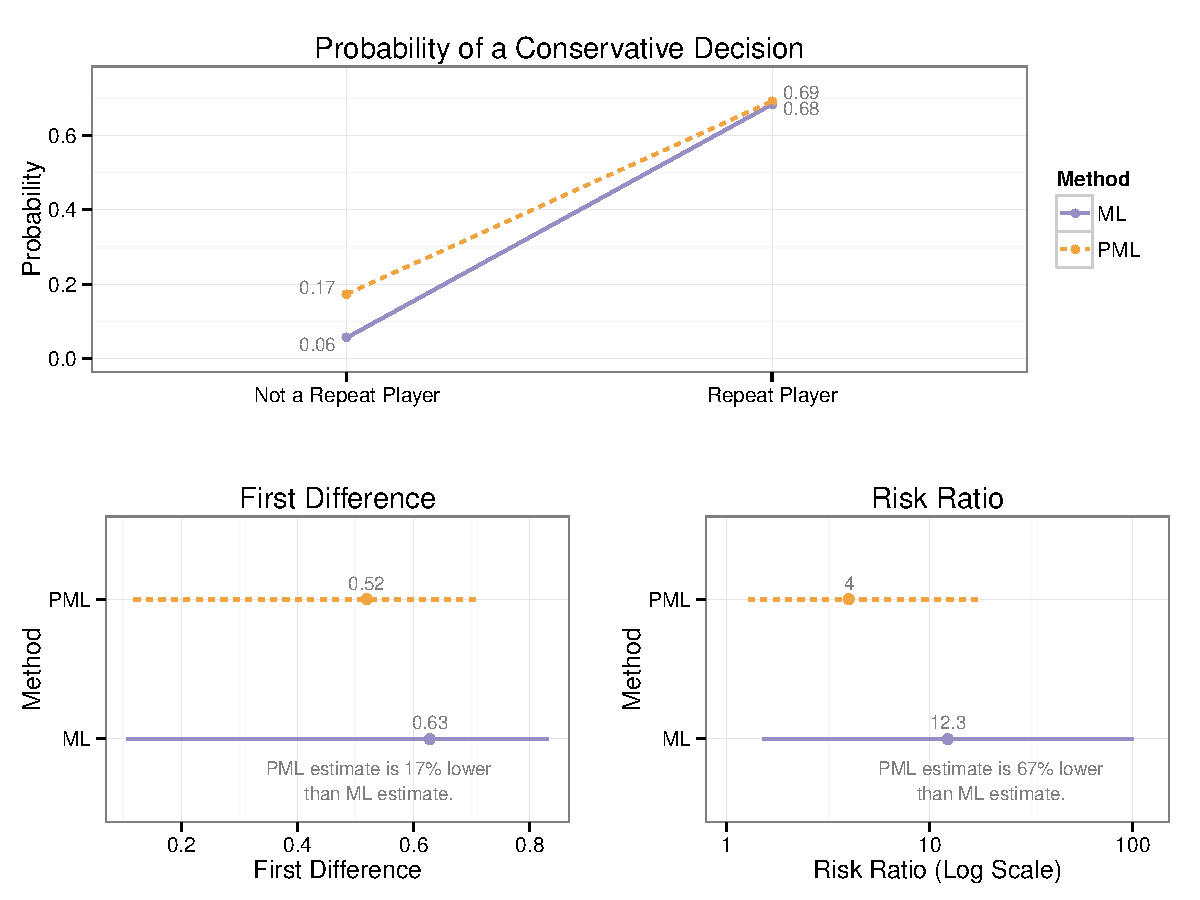
\includegraphics[width = \textwidth]{figs/ge-qis.pdf}
\caption{This figure shows the quantities of interest for the effect of the solicitor general filing a brief amicus curiae on the probability of a decision in favor of capital punishment.}\label{fig:ge-qis}
\end{center}
\end{figure}

Because we estimate a logit model, we are likely more interested in the functions of the coefficients rather than the coefficients themselves \citep{KingTomzWittenberg2000}.
For an example, we take George and Epstein's integrated model of Court decisions and calculate a first difference and risk ratio as the repeat-player status of the state varies, setting all other explanatory variables at their medians.
George and Epstein hypothesize that repeat players have greater expertise and are more likely to win the case.
Figure \ref{fig:ge-qis} shows the estimates of the quantities of interest.
\begin{figure}[h]
\begin{center}
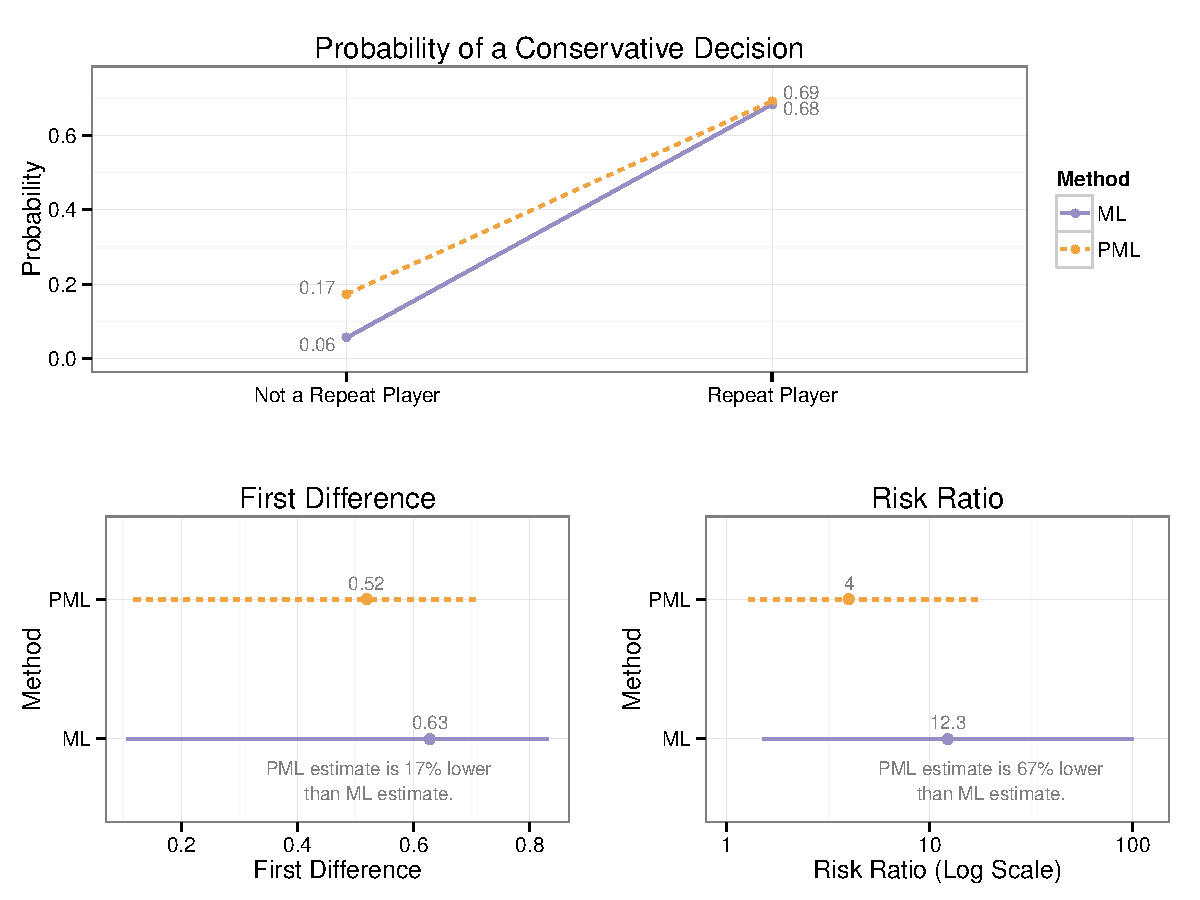
\includegraphics[width = \textwidth]{figs/ge-qis.pdf}
\caption{This figure shows the quantities of interest for the effect of the solicitor general filing a brief amicus curiae on the probability of a decision in favor of capital punishment.}\label{fig:ge-qis}
\end{center}
\end{figure}
The PML estimator pools the estimated probabilities toward one-half. When the state is not a repeat player, the PML estimates suggest a 17\% chance of a conservative decision while ML estimates suggest only a 6\% chance.
However, when the state is a repeat player, the PML estimates suggest that the Court has a 53\% chance of a conservative decision compared to the 60\% chance suggested by ML.
Thus, PML also provides smaller effect sizes for both the first difference and the risk ratio.
PML decreases the estimated first difference by 17\% from 0.63 to 0.52 and the risk ratio by 67\% from 12.3 to 4.0.

This example application clearly highlights the differences between the ML and PML estimators. 
The PML estimator shrinks the coefficient estimates and confidence intervals substantial. 
Theoretically, we know that these estimates have a smaller bias, variance, and MSE.
Practically, though, this shrinkage manifests in better out-of-sample predictions.
And these improvements come at almost \textit{no cost} to researchers. 
The PML estimator is nearly trivial to implement but \textit{dominates} the ML estimator--the PML estimator always has lower bias, lower variance, and lower MSE.

\section*{Recommendations to Substantive Researchers}

Throughout this paper, we emphasize one key point--when using small samples to estimate logit and probit models, the PML estimator offers a substantial improvement over the usual maximum likelihood estimator. 
But what actions should substantive researchers take in response to our methodological point? 
In particular, at what sample sizes should researchers consider switching from the ML estimator to the PML estimator?

\subsection*{Concrete Advice About Sample Sizes}

Prior research suggests two rules of thumb about sample sizes.
First, \cite{Peduzzietal1996} recommend about 10 events per explanatory variable, though \cite{VittinghoffMcCulloch2007} suggest relaxing this rule. 
Second, \citet[p. 54]{Long1997} suggests that ``it is risky to use ML with samples smaller than 100, while samples larger than 500 seem adequate.'' 
In both of these cases, the alternative to a logit or probit model seems to be no regression at all.
Here though, we present the PML estimator as an alternative, so we have room to make more conservative recommendations.
On the grounds that the PML estimator dominates the ML estimator, we might recommend that researchers always use the PML estimator. 
But we do not want or expect researchers to switch from the common and well-understood ML estimator to the PML estimator without a clear, meaningful improvement in the estimates.

We measure the cost of using ML rather than PML as the MSE inflation defined in Equation \ref{eqn:mse-infl}--the percent increase in the MSE when using ML rather than PML. 
The MSE inflation summarizes the relative inaccuracy of the ML estimator compared to the PML estimator.

To measure the information in a data set, we follow the biostatistics literature and use the number of events per explanatory variable $\frac{1}{k}\sum y_i$ (e.g., \citealt{Peduzzietal1996} and \citealt{VittinghoffMcCulloch2007}).
However, this approach assumes that events occur less often than non-events. 
To generalize this idea to a statistic more suitable to political science data, in which the number of events commonly exceeds the number of non-events, we use a measure of information $\xi$ that takes the minimum of the events and non-events per explanatory variable, so that
\begin{equation}
\xi = \frac{1}{k}\min \left[ \sum_{i = 1}^n y_i, \sum_{i = 1}^n(1 - y_i) \right]\text{ .}
\end{equation}

We use a Monte Carlo simulation to develop rules of thumb that link the amount of information $\xi$ to the cost of using ML rather than PML. 
The cost of using ML rather than PML decreases continuously with the amount of information in the data set, but to make concrete suggestions, we break the costs into three categories: substantial, noticeable, and negligible.
We use the following cutoffs.
\begin{enumerate}
\item \underline{Negligible}: If the MSE inflation probably falls below 3\%, then we refer to the cost as \textit{negligible}.
\item \underline{Noticeable}: If the MSE inflation of ML probably falls below 10\%, but not probably below 3\%, then we refer to the cost as \textit{noticeable}.
\item \underline{Substantial}: If the MSE inflation of ML might rise above 10\%, then we refer then the cost as \textit{substantial}.
\end{enumerate}

To develop our recommendations, we estimate the MSE inflation for a wide range of hypothetical analyses across which the true coefficients, the number of explanatory variables, and the sample size varies. 
To create each hypothetical analysis, we do the following:
\begin{enumerate}
\item Choose the number of covariates $k$ randomly from a uniform distribution from 3 to 12.
\item Choose the sample size $n$ randomly from a uniform distribution from 200 to 3,000.
\item Choose the intercept $\beta_{cons}$ randomly from a uniform distribution from -4 to 4.
\item Choose the slope coefficients $\beta_1,...,\beta_k$ randomly from a normal distribution with mean 0 and standard deviation 0.5.
\item Choose a covariance matrix $\Sigma$ for the explanatory variables randomly using the method developed by \cite{Joe2006} such that the variances along the diagonal range from from 0.25 to 2.
\item Choose the explanatory variables $x_1, x_2,...,x_k$ randomly from a multivariate normal distribution with mean 0 and covariance matrix $\Sigma$. 
\end{enumerate}
For each hypothetical analysis, we simulate 1,000 data sets and compute the MSE inflation of the ML estimator relative to the PML estimator using Equation \ref{eqn:mse-infl}.
We then use quantile regression to model the 90th percentile as a function of the information $\xi$ in the data set.
This quantile regression allows us to estimate the amount of information that researchers need to before the MSE inflation ``probably'' (i.e., about a 90\% chance) falls below some threshold.
We then calculate the thresholds at which the MSE inflation probably falls below 10\% and 3\%.

Interestingly, ML requires more information to estimate the intercept $\beta_{cons}$ accurately relative to PML than the slope coefficients $\beta_1,..., \beta_k$ (see \citealt{KingZeng2001}).
Because of this, we calculate the cutoffs separately from the intercept and slope coefficients.

If the researcher simply wants accurate estimates of the slope coefficients, then she risks substantial costs when using ML with $\xi \leq 12$ and noticeable costs when using ML with $\xi \leq 51$. If the researcher also wants an accurate estimate of the intercept, then she risks substantial costs when using ML with $\xi \leq 33$ and noticeable costs when using ML when $\xi \leq 96$. 

Importantly, the cost of ML only becomes negligible for all model coefficients when $\xi \geq 96$--this threshold diverges quite a bit from the prior rules of thumb.
For simplicity, assume the researcher wants to include eight explanatory variables in her model.
In the best case scenario of 50\% events, she should definitely use the PML estimator with fewer than $\frac{8 \times 12}{0.5} = 192$ observations and ideally use the PML estimator with fewer than $\frac{8 \times 51}{0.5} = 816$ observations.  
But if she would also like accurate estimates of the intercept, then these thresholds increase to $\frac{8 \times 33}{0.5} = 528$ and $\frac{8 \times 115}{0.5} = 1,536$ observations. 
Many logit and probit models estimated using survey data have fewer than 1,500 observations and these studies risk a noticeable cost by using a ML estimator rather than the PML estimator.
Further, these estimates assume 50\% events. 
As the number of events drifts toward 0\% or 100\% or the number of variables increases, then the researcher needs even more observations.

\begin{table}[h]
\centering
\begin{tabular}{ccc}
\hline
Acceptable Inaccuracy   &  Slopes Coefficients     & Intercept        \\ \hline
Substantial & $\xi < 12$         & $\xi < 33$          \\
Noticeable  & $12 \leq \xi < 51$ & $33 \leq \xi < 96$ \\
Negligible  & $\xi \geq 51$        & $\xi \geq 96$        
\end{tabular}
\caption{This table shows the thresholds at which the cost of ML relative to PML becomes substantial, noticeable, and negligible when estimating the slope coefficients and the intercept.}\label{tbl:thresholds}
\end{table}

\begin{figure}[h]
\begin{center}
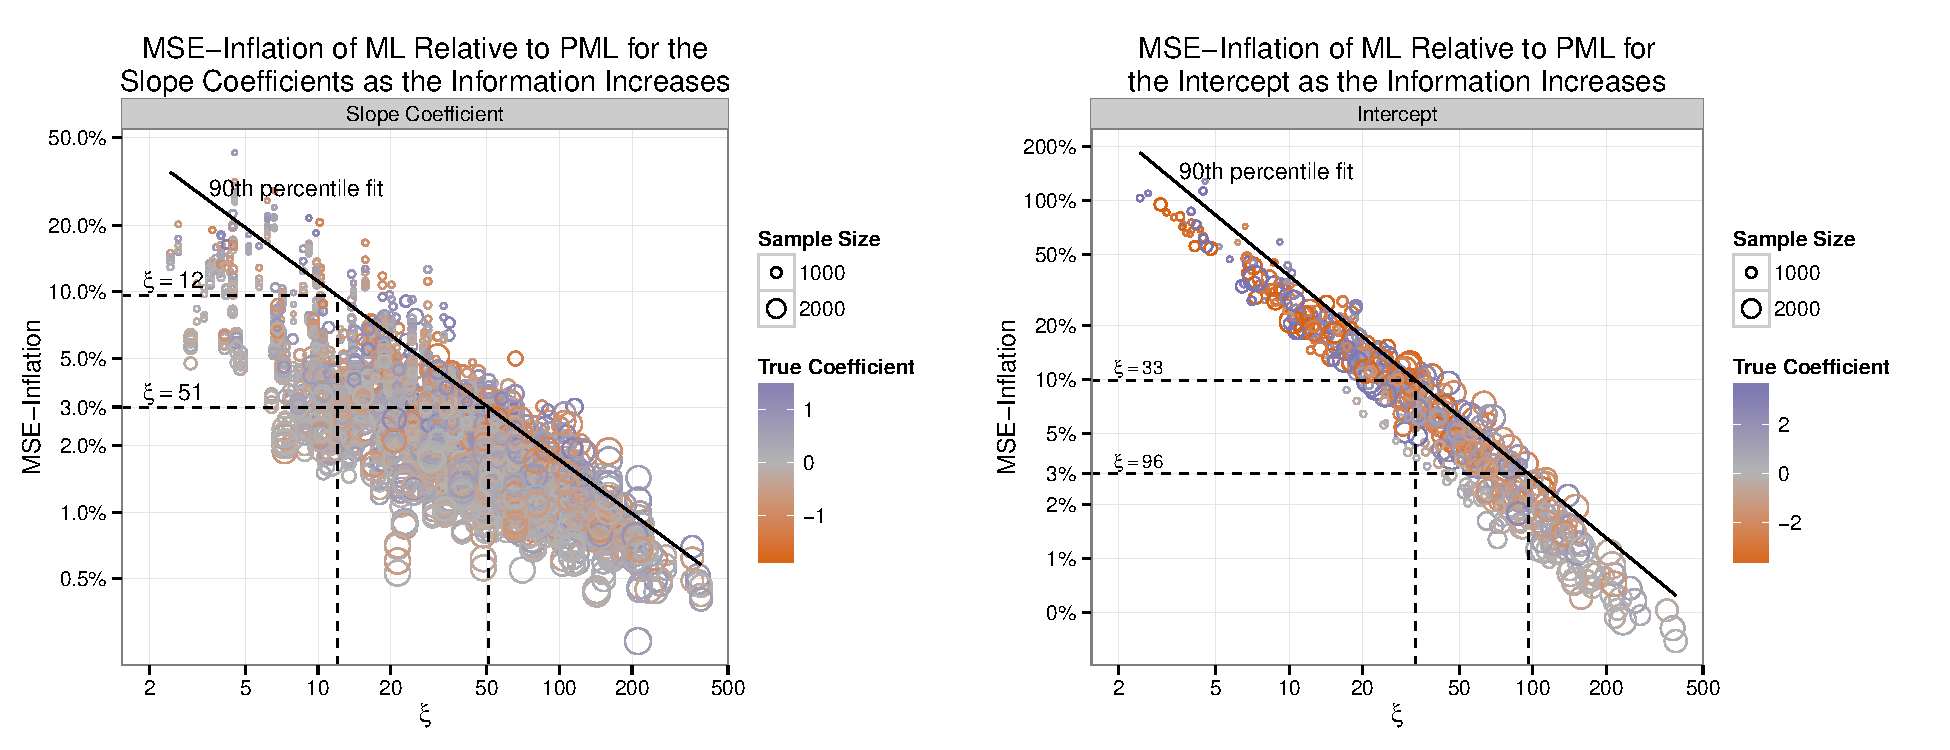
\includegraphics[width = \textwidth]{figs/mse-infl-larger-samples.pdf}
\caption{This figure shows the MSE inflation as the events per explanatory variable increases. The left panel shows the MSE inflation for the slope coefficients and the right panel shows the MSE inflation for the intercept.}\label{fig:ge-qis}
\end{center}
\end{figure}

\subsection*{Concrete Advice About Estimators}

When estimating a model of a binary outcome with a small sample, a researcher faces several options. 
First, she might avoid analyzing the data altogether because she realizes that maximum likelihood estimates of logit model coefficients have significant bias.
We see this as the least attractive option.
Even small data sets contain information and avoiding these data sets leads to a lost opportunity.

Second, the researcher might proceed with the biased and inaccurate estimation using maximum likelihood.
We also see this option as unattractive, because simple improvements can dramatically shrink the bias and variance of the estimates.

Third, the researcher might use least squares to estimate a linear probability model (LPM). If the probability of an event is a linear function of the explanatory variables, then this approach is reasonable, as long as the researcher takes steps to correct the standard errors.
However, in most cases, using an ``S''-shaped inverse-link function (i.e., logit or probit) makes the most theoretical sense, so that marginal effects shrink toward zero as the probability of an event approaches zero or one (e.g.,
%\citealt{Rainey2015};
\citealt{BerryDeMerittEsarey2010} and \citealt[pp. 34-47]{Long1997}).
\citet[p. 40]{Long1997} writes: ``In my opinion, the most serious problem with the LPM is its functional form.''
Additionally, the LPM sometimes produces nonsense probabilities that fall outside the $[0, 1]$ interval and nonsense risk ratios that fall below zero.
If the researcher is willing to accept these nonsense quantities and assume that the functional form is linear, then the LPM offers a reasonable choice.
However, we agree with \cite{Long1997} that without evidence to the contrary, the logit or probit model offers a more plausible functional form.

Finally, the researcher might simply use penalized maximum likelihood, which allows the theoretically-appealing ``S''-shaped functional form while greatly reducing the bias \textit{and} variance.
Indeed, the penalized maximum likelihood estimates always have a smaller bias and variance than the maximum likelihood estimates.
These substantial improvements come at almost no cost to the researcher in learning new concepts or software beyond maximum likelihood and simple commands in R and/or Stata.\footnote{Appendices \ref{sec:pmle-in-R} and \ref{sec:pmle-in-stata} offer a quick overview of computing penalized maximum likelihood estimates in R and Stata, respectively.}
We see this as the most attractive option.
Whenever researchers have concerns about bias and variance due to a small sample, a simple change to a penalized maximum likelihood estimator can easily ameliorate any concerns with little to no added difficulty for researchers or their readers.

\singlespace
\normalsize
\bibliographystyle{apsr_fs}
\bibliography{/Users/carlislerainey/Dropbox/papers/bibliography/bibliography.bib}
%\bibliography{/Users/kellymccaskey/Dropbox/projects/bibliography/bibliography.bib}

\newpage
\begin{appendix}
\begin{center}
{\LARGE Appendix}\\
\vspace{3mm}
{\large Estimating Logit Models with Small Samples}\\\vspace{2mm}
\end{center}

\section{PML Estimation in R}\label{sec:pmle-in-R}

This example code is available at \href{https://github.com/kellymccaskey/small/blob/master/R/example.R}{https://github.com/kellymccaskey/small/blob/master/R/example.R}.

\begin{footnotesize}
\begin{verbatim}

# load data from web
library(readr)  # for read_csv()
weisiger <- read_csv("https://raw.githubusercontent.com/kellymccaskey/small/master/weisiger-
	replication/data/weisiger.csv")

# quick look at data
library(dplyr)  # for glimpse()
glimpse(weisiger)

# model formula
f <- resist ~ polity_conq + lndist + terrain +
  soldperterr + gdppc2 + coord

# ----------------------------- #
# pmle with the logistf package #
# ----------------------------- #

# estimate logit model with pmle
library(logistf)  # for logistf()
m1 <- logistf(f, data = weisiger)

# see coefficient estimates, confidence intervals, p-values, etc.
summary(m1)

# logistf does **NOT** work with texreg package
library(texreg)
screenreg(m1)

# see help file for more
help(logistf)

# --------------------------- #
# pmle with the brglm package #
# --------------------------- #

# estimate logit model with pmle
library(brglm)  # for brglm()
m2 <- brglm(f, family = binomial, data = weisiger)

# see coefficient estimates, standard errors, p-values, etc.
summary(m2)

# brglm works with texreg package
screenreg(m2)

# see help file for more
help(brglm)
\end{verbatim}
\end{footnotesize}

\section{PML Estimation in Stata}\label{sec:pmle-in-stata}

This example code is available at \href{https://github.com/kellymccaskey/small/blob/master/stata/example.do}{https://github.com/kellymccaskey/small/blob/master/stata/example.do}.

\noindent The example data used is available at \href{https://github.com/kellymccaskey/small/blob/master/stata/GE.dta}{https://github.com/kellymccaskey/small/blob/master/stata/ge.csv}.

\begin{footnotesize}
\begin{verbatim}
* set working directory and load data
* data can be found at https://github.com/kellymccaskey/small/blob/master/stata/ge.csv
cd "your working directory"
insheet using "ge.csv", clear

* install firthlogit
ssc install firthlogit

* estimate logit model with pmle
* see coefficient values, standard errors, p-values, etc.
firthlogit court dq cr pc ag sp pe cc ap dc st sg

* see help file for more
help firthlogit

\end{verbatim}
\end{footnotesize}


\section{Additional Simulation Results}\label{sec:app-sims}

\subsection{Expected Value}

\begin{figure}[H]
\begin{center}
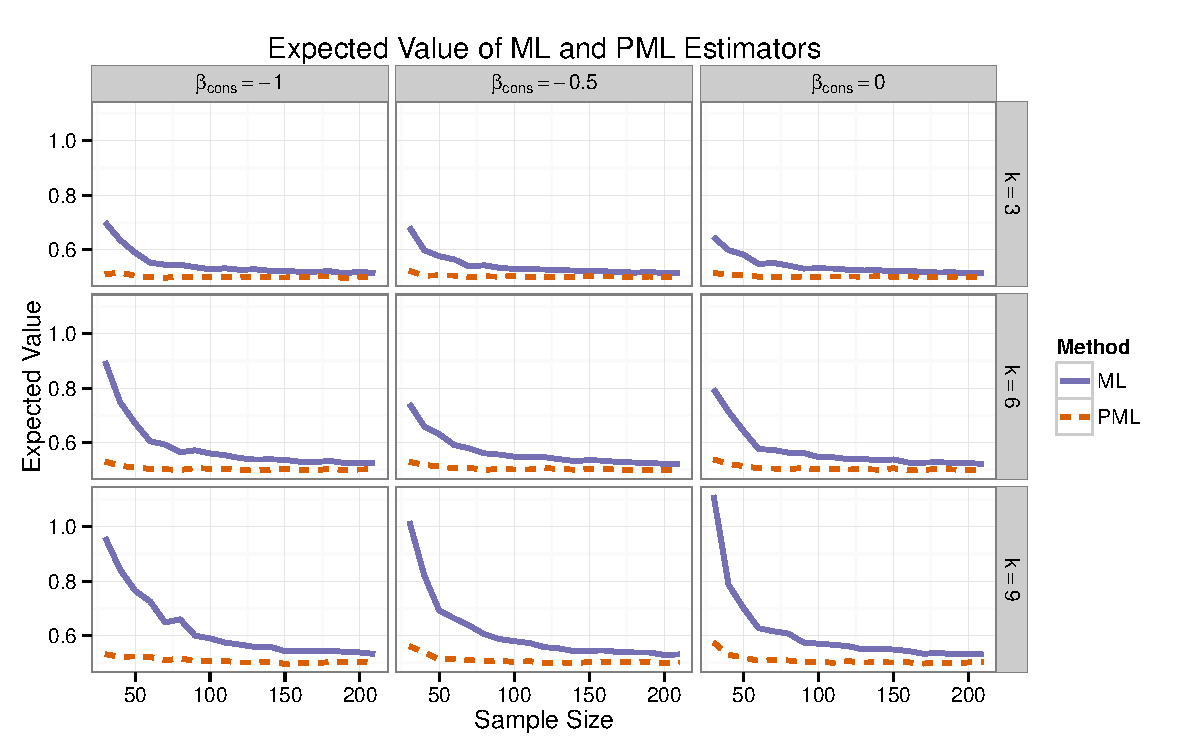
\includegraphics[width = \textwidth]{figs/sims-ev.pdf}
\caption{This figure shows the expected value of $\hat{\beta}^{mle}$ and $\hat{\beta}^{pmle}$. The true value is $\beta = 0.5$.}\label{fig:ev}
\end{center}
\end{figure}

\subsection{Bias}

\begin{figure}[H]
\begin{center}
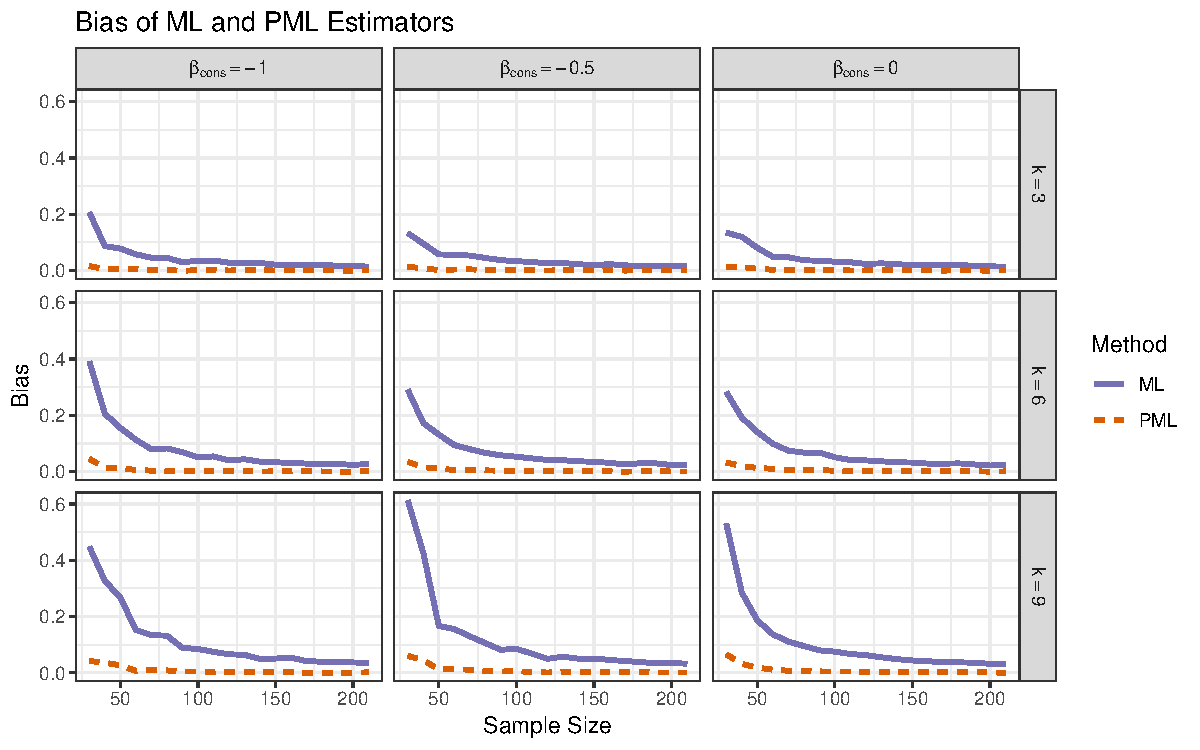
\includegraphics[width = \textwidth]{figs/sims-bias.pdf}
\caption{This figure shows the bias of $\hat{\beta}^{mle}$ and $\hat{\beta}^{pmle}$.}\label{fig:bias}
\end{center}
\end{figure}

\subsection{Variance Inflation}

\begin{figure}[H]
\begin{center}
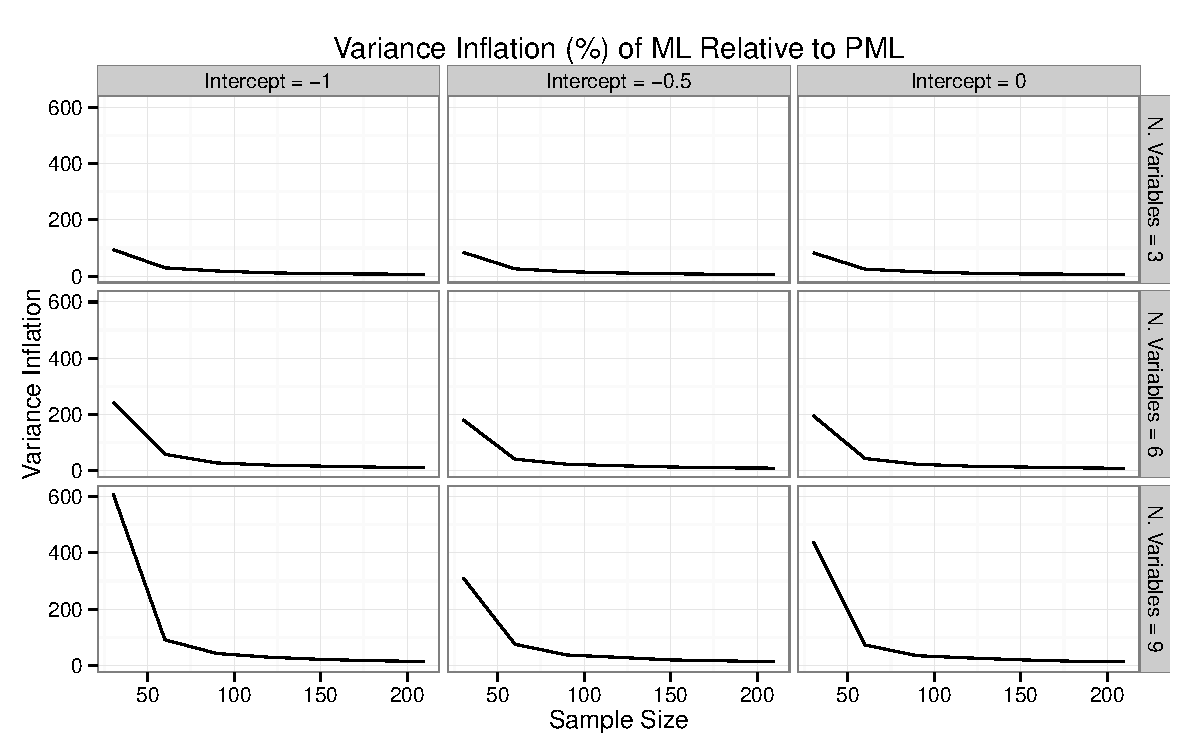
\includegraphics[width = \textwidth]{figs/sims-var-infl.pdf}
\caption{This figure shows the percent inflation in the variance of $\hat{\beta}^{mle}$ compared to $\hat{\beta}^{pmle}$.}\label{fig:var-infl}
\end{center}
\end{figure}

\section{Re-Analysis of \cite{Weisiger2014}}\label{app:weisiger}

Weisiger describes how, after the official end of the war, violence sometimes continues in the form of guerrilla warfare.
He argues that resistance is more likely when conditions are favorable for insurgency, such as difficult terrain, a occupying force, or a pre-war leader remains at-large in the country.

Weisiger's sample consists of 35 observations (with 14 insurgencies).
We reanalyze Weisiger's data using a logit model to show the substantial difference between the biased, high-variance ML estimates and the nearly unbiased, low-variance PML estimates.\footnote{Specifically, we reanalyze the Model 3 in Weisiger's Table 2 (p. 14).
In the original analysis, Weisiger uses a linear probability model.
He writes that ``I [Weisiger] make use of a linear probability model, which avoids problems with separation but introduces the possibility of non-meaningful predicted probabilities outside the [0,1] range'' (p. 11).
As he notes, predictions outside the $[0, 1]$ interval pose a problem for interpreting the linear probability model.
In these data for example, the linear probability model estimates a probability of 1.41 of insurgency in one case.
In another, it estimates a probability of -0.22.
Overall, 25\% of the estimated probabilities based on the linear probability model are larger than one or less than zero.
Of course, these results are nonsense.
However, because of the well-known small-sample bias, methodologists discourage researchers from using a logit model with small samples.
The PML approach, though, solves the problem of bias as well as nonsense predictions.} Prior to estimation, we standardize the continuous variables to have mean zero and standard deviation one-half and binary variables to have mean zero \citep{Gelman2008}.
Figure \ref{fig:weisiger-coefs} shows the coefficient estimates and 90\% confidence intervals using ML and PML.
Notice that the PML estimates are substantially smaller in many cases.
Although the coefficient for terrain only changes by 16\%, each of the remaining coefficients changes by more than 45\%!
The coefficient for per capita GDP shrinks by more the 60\% and the coefficient for occupying force density grows by nearly 100\%.
Also notice that the PML standard errors are much smaller--the ML estimates for the coefficients of a coordinating leader and for the intercapital distance fall outside the PML 90\% confidence interval.
On average, the PML confidence intervals are about half as wide as the ML confidence intervals.

\begin{figure}[h]
\begin{center}
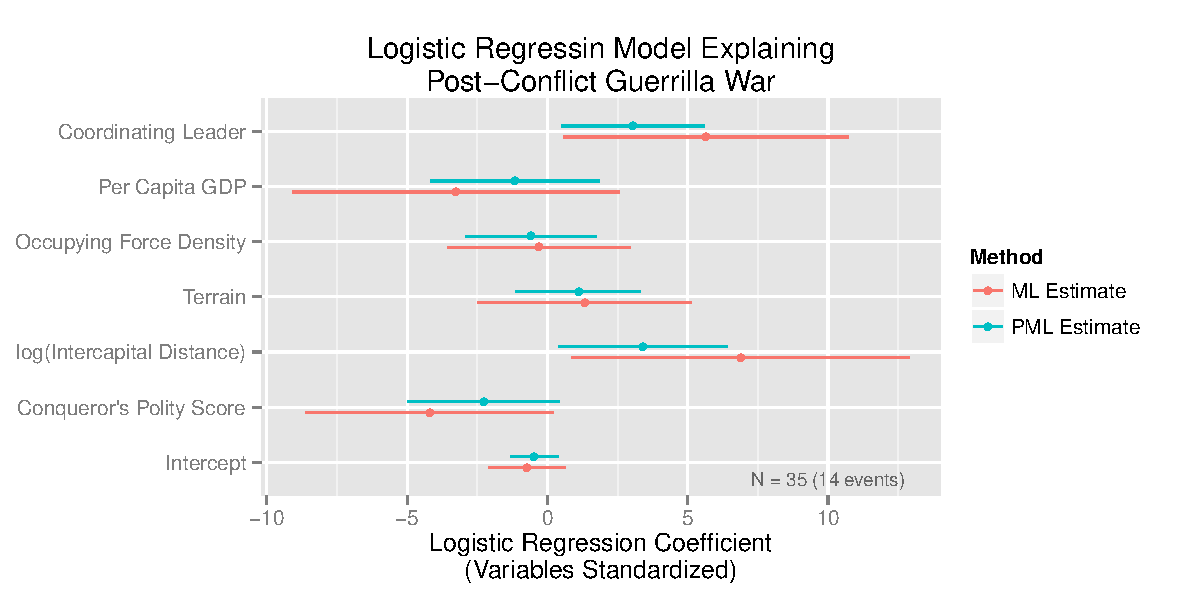
\includegraphics[width = \textwidth]{figs/weisiger-coefs.pdf}
\caption{This figure shows the coefficients for a logit model model estimated explaining post-conflict guerrilla war estimated with ML and PML.
Notice that the PML estimates and confidence intervals tend to be much smaller than the ML estimates and confidence intervals.}\label{fig:weisiger-coefs}
\end{center}
\end{figure}

Because we do not know the true model, we cannot know which of these sets of coefficients is better.
However, we can use out-of-sample prediction to help adjudicate between these two methods.
We use leave-one-out cross-validation and summarize the prediction errors using Brier and log scores, for which smaller values indicate better predictive ability.\footnote{The Brier score is calculated as $\sum_{i = 1}^n (y_i - p_i)^2$, where $i$ indexes the observations, $y_i \in \{0, 1\}$ represents the actual outcome, and $p_i \in (0, 1)$ represents the estimated probability that $y_i = 1$.
The log score as $-\sum_{i = 1}^n log(r_i)$, where $r_i = y_i p_i + (1 - y_i)(1 - p_i)$.
Notice that because we are logging $r_i \in [0, 1]$, $\sum_{i = 1}^n log(r_i)$ is always negative and smaller (i.e., more negative) values indicate worse fit.
We choose to take the negative of $\sum_{i = 1}^n log(r_i)$, so that, like the Brier score, larger values indicate a worse fit.}
The ML estimates produce a Brier score of 0.14, and the PML estimates lower the Brier score by 14\% to 0.12.
The ML estimates produce a log score of 0.58, while the PML estimates lower the log score by 34\% to 0.38.
The PML estimates outperform the ML estimates for both approaches to scoring, and
this provides good evidence that the PML estimates better capture the data generating process.

Because we are using a logit model, we might be more interested in \textit{functions} of the coefficients than in the coefficients themselves.
For an example, we focus on Weisiger's hypothesis that there will be a greater chance of resistance when the pre-conflict political leader remains at large in the conquered country.
Setting all other explanatory variables at their sample medians, we calculated the predicted probabilities, the first difference, and the risk ratio for the probability of a post-conflict guerrilla war as countries gain a coordinating leader.
Figure \ref{fig:weisiger-qis} shows the estimates of the quantities of interest.

\begin{figure}[h]
\begin{center}
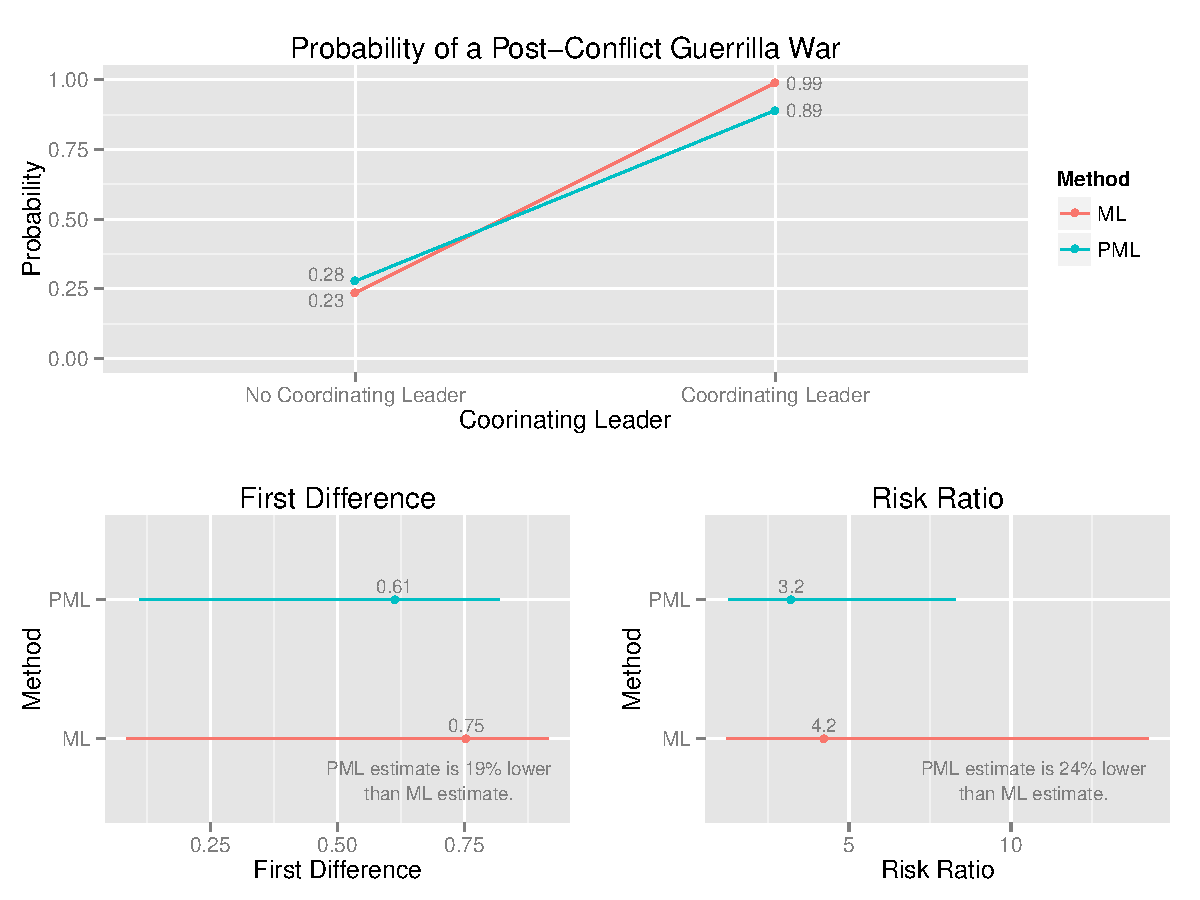
\includegraphics[width = \textwidth]{figs/weisiger-qis.pdf}
\caption{This figure shows the quantities of interest for the effect of a coordinating leader on the probability of a post-conflict guerrilla war.}\label{fig:weisiger-qis}
\end{center}
\end{figure}

PML pools the estimated probabilities toward one-half, so that when a country lacks a coordinating leader, ML suggests a 23\% chance of rebellion while PML suggests a 28\% chance.
On the other hand, when country \textit{does have} a coordinating leader, ML suggests a 99\% chance of rebellion, but PML lowers this to 89\%.
Accordingly, PML suggests smaller effect sizes, whether using a first difference or risk ratio.
PML shrinks the estimated first difference by 19\% from 0.75 to 0.61 and the risk ratio by 24\% from 4.2 to 3.2.

\end{appendix}


\end{document}
